\chapter{Results and Future Work}

\section{Experimental Results}

To evaluate the proposed method, we conducted experiments using the \textit{SummitXL} robot by \textit{Robotnik}, which is equipped with a laser scanner and IMU sensors. The test environment was a room measuring approximately $7 \times 6$ meters. We moved the robot slowly to minimize noise in the data collected by the IMU.

\begin{figure}[H]
    \centering
    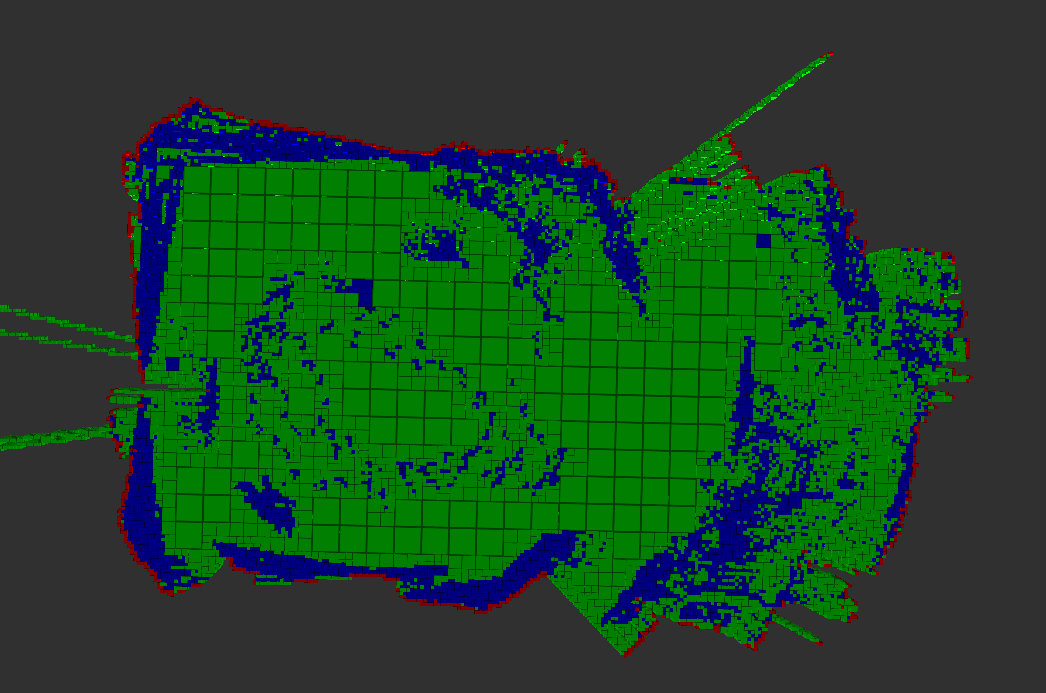
\includegraphics[width=\textwidth]{images/top_screenshot.png}
    \caption{Top view of the octomap generated by our program in the P.E.R.M.I.S. environment. The gray area represents unknown space, the green area represents free space, and the red area represents occupied space. Only the major probability values are shown.}
\end{figure}

In the P.E.R.M.I.S. environment, using the \textit{SummitXL} robot, we obtained the following results:

\begin{itemize}
    \item The octomap provides a coherent representation of the environment, with the boundaries of the room clearly defined.
    \item Moving objects are detected; in the figure, the circle made of blue points represents a person moving around.
    \item Near the room boundaries, the program detects numerous conflicts, likely due to the robot's movement and IMU imperfections.
    \item Attenuation could be useful for detecting moving objects. Occupied cells surrounded by conflict cells often indicate a fixed object, whereas disappearing conflicts usually indicate a moving object.
    \item The program runs in real-time at approximately 15 Hz and could be significantly improved by reducing the resolution.
\end{itemize}

\section{Future Work}

The proposed implementation is a first step towards using Evidential Grids for detecting moving objects. However, several improvements are needed to enhance its efficiency and reliability.

\subsection{Implementation Improvements}

Firstly, the program can be optimized for faster performance, potentially by using GPUs. Due to time constraints, we couldn't implement a tiled system to reduce memory usage. The lack of standardization in ROS messages is also problematic, as different robot manufacturers do not use the laser scan message uniformly. This prevented us from implementing a robust system to filter reliable data. We considered creating or using a more suitable message to transmit the EOGM data. One idea is to use an existing message for Rviz and another for other nodes. Additionally, developing a new message with its own Rviz plugin is a possibility.

\subsection{Methodological Improvements}

Methodologically, the IMU data is very noisy due to the robot's movements, resulting in a high area of conflict. One solution could be to use a better IMU or to find a way to reduce conflicts near fixed objects.
Maybe SLAM algorithms could be used to improve the robot's localization and reduce conflicts. The robot's movement could also be used to detect moving objects. For example, if the robot moves forward and the conflict disappears, it could indicate a moving object. The robot's movement could also be used to detect the robot's position and orientation, which could be used to improve the robot's localization.
